% filepath: /home/teus/github/CursinhoEACH/doc/documentacao.tex
\documentclass{article}
\usepackage[a4paper,margin=2cm]{geometry}
\usepackage{amsmath}
\usepackage{diagbox}
\usepackage{graphicx}    
\graphicspath{{figures/}}

\title{EP Banco de Dados 1 - EACH Cursinho}
\author{
    \begin{tabular}{r l}
        Alexsandro de Souza Campos & 15493520 \\
        Arthur Almeida Betti & 15586631 \\
        Matheus Machado Alfradique & 8957120 \\
        Matheus Silva Portes de Lima & 15479684 \\
    \end{tabular}
}
\date{\today}

\begin{document}
\maketitle

\section{Domínio e Minimundo}
O trabalho realizado pelo grupo possui como domínio o Cursinho Popular da EACH - USP, nosso minimundo representa uma simplificação do escopo de suas atividades, abstraindo as principais demandas e necessidades funcionais em nosso sistema. 

Ao fim do trabalho, nosso objetivo é apresentar um protótipo funcional que será incrementado ao longo das demais matérias da graduação. As aplicações desenvolvidas nessa disciplina de banco de dados visam auxiliar a entidade nas seguintes tarefas operacionais: controle e acompanhamento da assiduidade e desempenho dos estudantes nas aulas, simulados e vestibulares ao longo do ano, disponibilizando dados e análises de forma personalizada à gestão pedagógica do CPE.

\section{Requisitos de Dados}

Uma instituição de ensino deseja construir um sistema de gerenciamento acadêmico completo. A base do sistema é o cadastro de Pessoas, onde para cada uma deve-se registrar informações essenciais como CPF (único), nome, e-mail, telefone, endereço e data de nascimento. O sistema também deve gerenciar o vínculo de Representante Legal, associando uma Pessoa (o responsável) a outra Pessoa (o aluno).

Uma Pessoa no sistema pode ser classificada como Aluno ou Professor. Para cada Aluno, é necessário armazenar seu ano escolar e informações de status, como se está matriculado ou o motivo de um eventual desligamento. Um Aluno deve pertencer a uma e somente uma Turma, enquanto uma Turma pode ter vários Alunos ou mesmo nenhum.

Para um Professor, é preciso definir seu tipo de vínculo com a instituição. Um Professor pode lecionar várias combinações de Matéria e Turma. Matéria é lecionada por várias combinações de Professor e Turma. Turma participa de várias combinações entre Professor e Matéria.

A organização estrutural é feita em Turmas, definidas por seu período, ano e capacidade máxima. O conteúdo programático é dividido em Matérias, que possuem um nome (único) e pertencem a uma área de conhecimento. 

O calendário acadêmico é composto por Eventos, cada qual com um ID (único), data, hora de início e duração. Um Evento está associado a no máximo uma Matéria. As avaliações são formalizadas como Provas, que possuem um ID (único), nome e fase. Uma mesma Prova pode ser aplicada em um ou mais Eventos distintos (por exemplo, em diferentes datas para turmas diferentes).

Uma Prova é composta por várias Questões, e uma mesma Questão pode ser reutilizada em múltiplas Provas. Cada Questão possui seu identificador único e o gabarito.

Quando um Aluno realiza uma Prova, o sistema deve registrar cada Resposta que ele fornece a uma Questão específica. Para cada Resposta, armazena-se a alternativa escolhida e o tempo de resposta, criando um vínculo que conecta unicamente um Aluno, uma Questão e uma Prova.


\section{Requisitos Funcionais}

\subsection{Alerta Evasão}

Alertas automáticos referentes a alunos com baixa frequência e risco de evasão escolar. Disparo de e-mail semanal ao corpo pedagógico com a lista de alunos e suas respectivas métricas de evasão. 
\vspace{0.5cm}

\textbf{Métricas de evasão:}

\begin{itemize}
    \item Frequência em simulados (último simulado, média móvel)
    \item Frequência em aulas (média semanal, média móvel)
    \item Risco de evasão: classificação do risco de evasão com base nas frequências em aulas e simulados categorizados em alto, médio e baixo. Índice de assiduidade em aulas (IAA) e índice de assiduidade em simulados (IAS).
\end{itemize}
\[
IAA = \frac{\text{Total de Aulas com Presença do Aluno}}{\text{Total de Aulas Ministradas para a Turma no Período}} \times 100
\]

\[
IAS = \frac{\text{Total de Simulados Obrigatórios que o Aluno Participou}}{\text{Total de Simulados Obrigatórios Aplicados no Período}} \times 100
\]

\begin{table}[h!]
    \centering
    \caption{Classificação de Risco de Evasão (Produto Cartesiano IAS × IAA)}
    \begin{tabular}{|c|c|c|c|}
    \hline
    \diagbox{IAS}{IAA} & $]85, 100]$ & $[65, 85]$ & $[0, 65[$ \\
    \hline
    $]80, 100]$  & Risco baixo & Risco médio & Risco médio \\
    $[50, 80]$   & Risco baixo & Risco médio & Risco alto  \\
    $[0, 50[$    & Risco médio & Risco alto  & Risco alto  \\
    \hline
    \end{tabular}
\end{table}

\subsection{Painel Meus Alunos}

Painel interativo com informações harmonizadas de todos os alunos. Permite consultas interativas sobre o desempenho e assiduidade de um aluno ou grupo de alunos a partir de critérios definidos pelos usuários (setor pedagógico). 
\vspace{0.5cm}

\textbf{Métricas de desempenho:}

\begin{itemize}
    \item Valor absoluto do número de acertos por área do conhecimento e prova.
    \item Nota média do aluno por simulado, tanto média global quanto segregada por área.
    \item Valor absoluto de questões deixadas em branco por simulado. Porcentagem de questões em branco.
\end{itemize}
\vspace{1cm}

\textbf{Métricas de assiduidade:}
\begin{itemize}
    \item Número de faltas por matéria com filtro de período, disciplina e docente.
    \item Número de simulados realizados.
\end{itemize}

\subsection{Painel Simulados}

Painel interativo com informações harmonizadas sobre simulados aplicados a fim de avaliar a taxa de aderência e viabilidade da aplicação do mesos. Permite consultas interativas sobre o engajamento dos alunos em simulados a partir de critérios definidos pelos usuários (corpo pedagógico).
\vspace{0.5cm}

\textbf{Estatísticas fixas:}
\begin{itemize}
    \item Nota média da turma por matéria.
    \item Nota média da turma no simulado.
    \item Percentual de evolução da turma no simulado comparado com demais simulados.
    \item Presença dos alunos por dia.
    \item Taxa de questões respondidas por aluno (\% de questões deixadas em branco).
\end{itemize}

\section{Diagrama Conceitual}
\begin{figure}[h!]
    \centering
    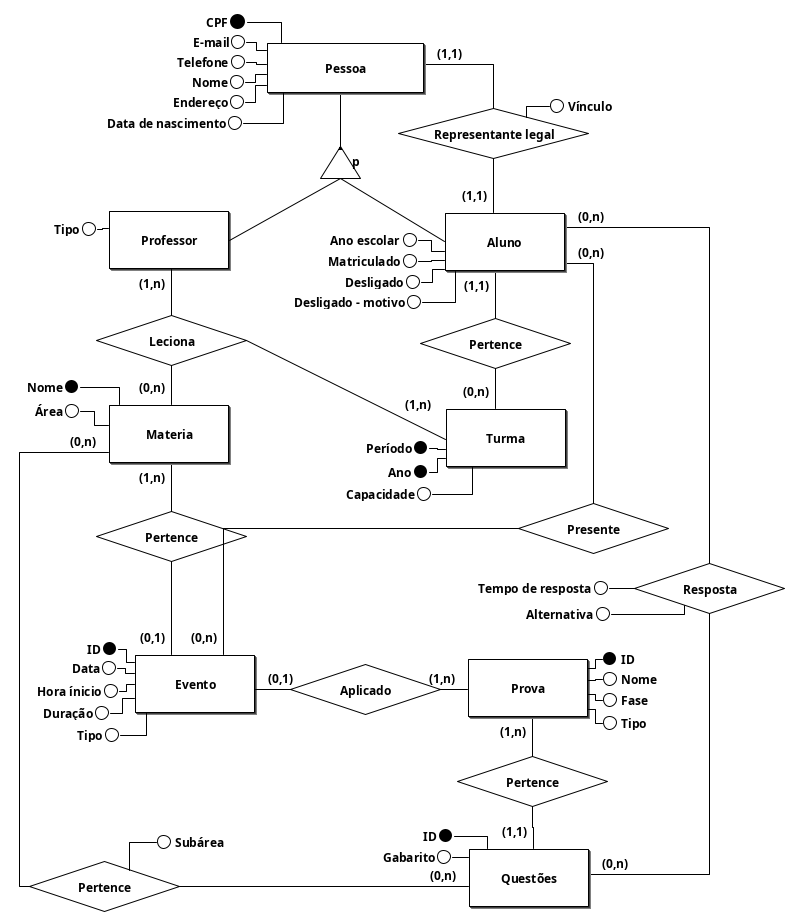
\includegraphics[width=0.8\textwidth]{Conceitual_1.png} 
    \caption{Modelo Conceitual}
    \label{fig:myimage}
\end{figure}


\end{document}